\section{Nguyên tố hóa học}
\begin{Muctieu}
	\begin{itemize}
		\item  Trình bày được khái niệm về nguyên tố hoá học, số hiệu nguyên tử, số khối và kí hiệu nguyên tố tưu.
		\item  Phát biểu được khái niệm đồng vị, nguyên tử khối.
		\item  Tính được nguyên tử khối trung bình (theo amu) dựa vào khối luợng nguyên tử và phần trăm số nguyên tử của các đồng vị theo phổ khối lượng được cung cấp.
	\end{itemize}
\end{Muctieu}
\begin{kd}
	\immini{Trên nhãn chai, chúng ta thấy nhiều ký hiệu hóa học như Ca, Mg, Na. Đây chính là các nguyên tố hóa học đang hiện diện trong cuộc sống hàng ngày của chúng ta. Mỗi nguyên tố này đều có vai trò riêng, tạo nên đặc tính của nước và ảnh hưởng đến sức khỏe chúng ta. Hôm nay, chúng ta sẽ cùng nhau tìm hiểu sâu hơn về những nguyên tố hóa học này và khám phá thế giới kỳ diệu của chúng. Vậy nguyên tố hóa học là gì? Chúng có những đặc điểm gì? Và tại sao việc hiểu về chúng lại quan trọng đến vậy? Hãy cùng bắt đầu bài học của chúng ta}{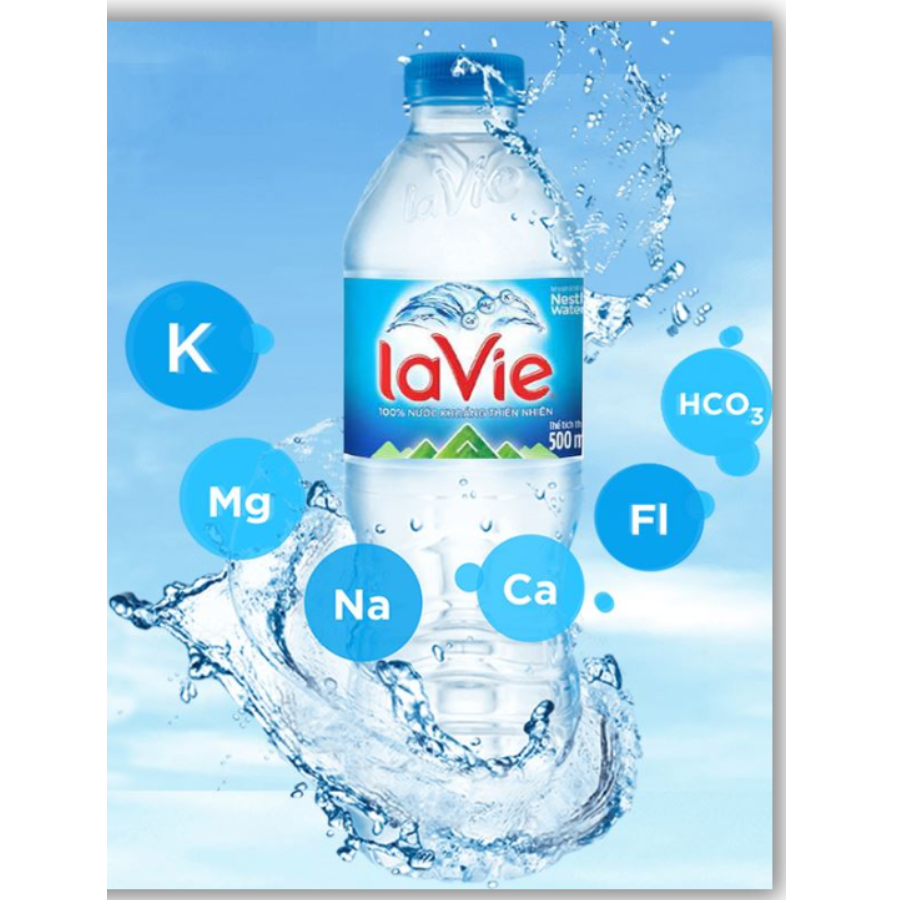
\includegraphics[width=4cm]{Images/anhhoahoc10/nuockhoang.png}}
\end{kd}
\subsection{Nội dung bài học}
	\subsubsection{Nguyên tố hóa học}
\begin{paracol}{2}
	\Noibat{Khái niệm nguyên tố hóa học}
	\vspace{0.5cm}
	\begin{tomtat}
		\indam{Nguyên tố hoá học} là tập hợp các nguyên tử có \indam{cùng số đơn vị điện tích hạt nhân} nhưng khác nahu về số neutron. Trong nguyên tử, số đơn vị điện tích hạt nhân bằng số electron ở vỏ nguyên tử. Các electron trong nguyên tử quyết định tính chất hoá học của nguyên tử, nên các nguyên tử của cùng một nguyên tố hoá học có \indam{tính chất hoá học giống nhau}.
	\end{tomtat}
	\switchcolumn
	\begin{Bancobiet}
		Cho đến năm 2020, đã có \indam{118} nguyên tố hoá học được xác định, trong đó \indam{94} nguyên tố có nguồn gốc \indam{tự nhiên}, còn lại là nguyên tớ nhân tạo. Nguyên tố phố biến nhất ở lớp vỏ Trái Đất là oxygen $(\mathrm{O})$, chiếm khoảng $46,6 \%$ khối lượng, tiếp theo là silicon (Si) chiếm khoảng 27,7\% khối lượng.
	\end{Bancobiet}
\end{paracol}
%%%
\Noibat{Số hiệu nguyên tử, số khối, kí hiệu nguyên tử}
\begin{tomtat}
	\begin{enumerate}
		\item Số proton trong hạt nhân được gọi là \indam{số hiệu nguyên tử}.
		\begin{vidu}
			Hạt nhân nguyên tử Oxigen có 8 proton, vậy số hiệu nguyên tử của O là 8 ($Z_{O}=8$)
		\end{vidu}
		\item Tổng số proton ($Z$) và neutron ($N$) trong một hat nhân gọi là \indam{số khối}, kí hiệu là A.
		\[\hopcttoan{\mathsf{A=Z+N}}\]
		\item Kí hiệu nguyên tử $_Z^AX$ cho biết kí hiệu  hóa học của nguyên tố ($X$), số hiệu nguyên tử ($Z$) và số khối ($A$).
		\begin{center}
			\begin{tikzpicture}[declare function={d=1.5;},line cap=round,line join=round]
				\tikzstyle{stylenode} = [color=\maunhan,font=\bfseries\fontsize{25pt}{6pt}\fontfamily{qag}\selectfont,inner sep=3pt,outer sep = 3pt]
				\tikzstyle{stylenodeH} = [anchor=east,color=\maunhan!30!black,font=\bfseries\fontsize{14pt}{0pt}\fontfamily{qag}\selectfont,xshift=2pt,inner sep=3pt,outer sep = 3pt]
				\tikzstyle{stylenodeB} = [font=\small,text width =3cm,inner sep=3pt,outer sep = 3pt]
				%%%
				\path (0,0) node[stylenode] (KHHH) {Al};
				\path (KHHH.north west) node [stylenodeH] (sk) {27};
				\path (KHHH.south west) node [stylenodeH] (shnt) {13};
				\path ($(KHHH)+(d,0)$) node [stylenodeB,anchor=west] (khhh) {Kí hiệu hóa học của nguyên tố};
				\path ($(sk)+({-0.8*d},0)$) node [stylenodeB,anchor=east,align=right] (SK) {Số khối};
				\path ($(shnt)+({-0.8*d},0)$) node [stylenodeB,anchor=east,align=right] (SHNT) {Số hiệu nguyên tử};
				%%%
				\path [fill=\maunhan,rounded corners =4pt,fill opacity=.2] (sk.north west)-|(KHHH.east)|-(shnt.south west)--cycle;
				%%%
				\foreach \x/\y in {KHHH/khhh,SHNT/shnt,SK/sk}
				{\path [draw=\maunhan,thick,shorten <=-0.1cm,shorten >=-0.15cm] (\x)--(\y);}
			\end{tikzpicture}
			\captionof{figure}{Kí hiệu nguyên tử Aluminium}\label{fig:KHHHAl}
		\end{center}
	\end{enumerate}
\end{tomtat}
\subsubsection{Đồng vị, nguyên tử khối trung bình}
\Noibat{Đồng vị}\\
Các nguyên tử của cùng một nguyên tố hóa học có số neutron khác nhau  là đồng vị của nhau
\begin{vidu}[\maunhan]
	Ba loại nguyên tử Oxigen $(\mathrm{O})$ đều có cùng 8 proton trong hạt nhân nên thuộc cùng một nguyên tố hoá học, nguyên tố oxigen $(\mathrm{O})$.
	\begin{center}
		\begin{tikzpicture}[line join=round,line cap=round]
			\tikzset{%
				pics/.cd,
				hinhcau/.style args={#1}{%
					code={\path[pic actions] circle (#1 pt);}
				},
				quydao/.style args={#1}{%
					code={\path[even odd rule,pic actions] circle (#1 cm) circle 	(#1 cm-2pt);}
				}
			}
			%%%===Đồng vị 16========%%%
			\path (0,0) node (m) {\tikz{
					\foreach \p/\m in {
						(0,0)/\maunhan,(45:5pt)/\maunhan,
						(-45:5pt)/\mauphu,(90:5pt)/\mauphu,
						(0:5pt)/\mauphu,(180:5pt)/\mauphu,
						(-135:6pt)/\maunhan,(135:6pt)/\maunhan,
						(-90:7pt)/\maunhan,(90:8pt)/\mauphu,
						(0:8pt)/\maunhan,(180:8pt)/\mauphu,
						(-90:5pt)/\mauphu,(45:8pt)/\maunhan,
						(-30:10pt)/\mauphu,(135:10pt)/\maunhan
					}{
						\path \p pic[ball color=\m] {hinhcau={3}};
					}
					\path (0,0) pic[fill=\maunhan!30]{quydao={1.4}};
					\path (0,0) pic[fill=\maunhan!30]{quydao={1.8}};
					%%%Electron%%%
					%%lop1
					\foreach \g in {0,180}{
						\path (\g:{1.4cm-1pt}) pic[ball color=gray!60!white] {hinhcau={2}};
					}
					%%lop2
					\foreach \g in {45,105,165,215,275,335}{
						\path (\g:{1.8cm-1pt}) pic[ball color=gray!60!white] {hinhcau={2}};
					}
			}};
			%%%===Đồng vị 17========%%%
			\node[right=2cm of m] (h) {\tikz{
					\foreach \p/\m in {
						(0,0)/\mauphu,(45:5pt)/\maunhan,
						(-45:5pt)/\mauphu,(90:5pt)/\maunhan,
						(0:5pt)/\mauphu,(180:5pt)/\maunhan,
						(-135:6pt)/\maunhan,(135:6pt)/\mauphu,
						(-90:7pt)/\maunhan,(90:8pt)/\mauphu,
						(0:8pt)/\mauphu,(180:8pt)/\maunhan,
						(-90:5pt)/\maunhan,(45:8pt)/\mauphu,
						(-30:10pt)/\mauphu,(135:10pt)/\maunhan,
						(-135:11pt)/\mauphu
					}{
						\path \p pic[ball color=\m] {hinhcau={3}};
					}
					\path (0,0) pic[fill=\maunhan!30]{quydao={1.4}};
					\path (0,0) pic[fill=\maunhan!30]{quydao={1.8}};
					%%%Electron%%%
					%%lop1
					\foreach \g in {0,180}{
						\path (\g:{1.4cm-1pt}) pic[ball color=gray!60!white] {hinhcau={2}};
					}
					%%lop2
					\foreach \g in {45,105,165,215,275,335}{
						\path (\g:{1.8cm-1pt}) pic[ball color=gray!60!white] {hinhcau={2}};
					}
					
			}};
			%%%===Đồng vị 18========%%%
			\node [right=2cm of h] (b) {\tikz{
					\foreach \p/\m in {
						(0,0)/\mauphu,(45:5pt)/\maunhan,
						(-45:5pt)/\mauphu,(90:5pt)/\maunhan,
						(0:5pt)/\mauphu,(180:5pt)/\maunhan,
						(-135:6pt)/\maunhan,(135:6pt)/\mauphu,
						(-90:7pt)/\maunhan,(90:8pt)/\mauphu,
						(0:8pt)/\mauphu,(180:8pt)/\maunhan,
						(-90:5pt)/\maunhan,(45:8pt)/\mauphu,
						(-30:10pt)/\mauphu,(135:10pt)/\maunhan,
						(-135:11pt)/\mauphu,(90:11pt)/\mauphu
					}{
						\path \p pic[ball color=\m] {hinhcau={3}};
					}
					\path (0,0) pic[fill=\maunhan!30]{quydao={1.4}};
					\path (0,0) pic[fill=\maunhan!30]{quydao={1.8}};
					%%%Electron%%%
					%%lop1
					\foreach \g in {0,180}{
						\path (\g:{1.4cm-1pt}) pic[ball color=gray!60!white] {hinhcau={2}};
					}
					%%lop2
					\foreach \g in {45,105,165,215,275,335}{
						\path (\g:{1.8cm-1pt}) pic[ball color=gray!60!white] {hinhcau={2}};
					}
			}};
			%%%=====Ghi chú ============
			\path(h.south) node [anchor=north,yshift=-1cm] {\tikz{
					\path (0,0) pic[ball color=gray!60!white,local bounding box=e] 	{hinhcau={4}};
					\node [right= 3pt of e] (electron) {Electron};
					\path ($(electron.east)+(1cm,0)$) pic[ball color=\maunhan,local 	bounding box=p] {hinhcau={6}};
					\node [right= 3pt of p] (proton) {Proton};
					\path ($(proton.east)+(1cm,0)$) pic[ball color=\mauphu,local 	bounding box=n] {hinhcau={6}};
					\node [right= 3pt of n] (notron) {Neutron};
			}};
			%%%===Tên đồng vị===========%%%
			\path (m.south) node[anchor=north,font=\color{\maunhan}\bfseries\small\sffamily]{Đồng vị $_{\phantom{1}8}^{16}O$};
			\path (h.south) node[anchor=north,font=\color{\maunhan}\bfseries\small\sffamily]{Đồng vị $_{\phantom{1}8}^{17}O$};
			\path (b.south) node[anchor=north,font=\color{\maunhan}\bfseries\small\sffamily]{Đồng vị $_{\phantom{1}8}^{18}O$};
		\end{tikzpicture}
		\captionof{figure}{Ba đồng vị phổ biến của Oxigen}
		\label{fig:dongvioxi}
	\end{center}
\end{vidu}
\Noibat{Nguyên tử khối trung bình}
\Noibat[][][\faArrowCircleOLeft]{Nguyên tử khối}

Nguyên tử khối là \indam{khối lượng tương đối} của một nguyên tử, cho biết nguyên tử đó nặng gấp bao nhiêu lần 1 \indam{amu}\footnote{Viết tắt của cụm từ \lq\lq atom mass unit \rq\rq}.

\Noibat[][][\faArrowCircleOLeft]{Nguyên tử khối trung bình}

\indam{Công thức tính nguyên tử khối trung bình:}
\hopcttoan{\overset{\resizebox{0.27cm}{!}{\_}}{\mathsf{A}}=\frac{\mathsf{X} \cdot \mathsf{x}+\mathsf{Y} \cdot \mathsf{y}+\mathsf{Z} \cdot \mathsf{z}+\ldots}{\mathsf{x}+\mathsf{y}+\mathsf{Z}}}\\
Trong đó :
\begin{itemize}
	\item X, Y, Z, $\ldots$ lần lượt là số khối của các đồng vị
	\item x, y, z ,$\ldots$ là phần trăm số nguyên tử các đồng vị tương ứng.
\end{itemize}
\begin{tongket}{Em đã học}
	\begin{itemize}
		\item  Nguyên tố hoá học là tập hợp các nguyên tử có cùng số đơn vị điện tích hạt nhân.
		\item  Đồng vị là những nguyên tử có cùng số đơn vị điện tích hạt nhân (cùng số proton) nhưng có số neutron khác nhau.
		\item  Kí hiệu của nguyên tử: $\mathrm{Z} X$.
		\item  Nguyên tử khối cho biết khối lượng nguyên tử đó nặng gấp bao nhiêu lần đơn vị khối lượng nguyên tử.
		\item  Nguyên tử khối của một nguyên tố là nguyên tử khối trung bình của hỗn hợp các đồng vị của nguyên tố đó.
	\end{itemize}
\end{tongket}
\subsection{Các dạng bài tập}
	\begin{dang}{Lý thuyết về nguyên tố hóa học}\end{dang}
\begin{pp}
	Nắm vững khái niệm về nguyên tố, đồng vị, nguyên tử khối trung bình.
\end{pp}
%%%Ví dụ mẫu dạng 1%%%
\Noibat[\maunhan][][\faBookmark]{Ví dụ mẫu}
%%%=============VDM 1=============%%%
%%%==============Cau_VDEX1==============%%%
\begin{vdex}
	Số hiệu nguyên tử cho biết thông tin nào sau đây?
	\choice
	{\True Số proton}
	{Số neutron}
	{Số khối}
	{Nguyên tử khối}
	\loigiai{
	Số hiệu nguyên tử bằng số đơn vị điện tích hạt nhân, bằng số proton.
	}
\end{vdex}
%%%==============HetCau_VDEX1==============%%%
%%%==============Cau_VDEX2==============%%%
\begin{vdex}
	Kí hiệu nguyên tử nào sau đây viết đúng?
	\choice
	{\True $_{\phantom{7}7}^{15}\mathrm{N}$}
	{$^{16}O$}
	{$16S$}
	{$\mathrm{Mg}_{12}^{24}$}
	\loigiai{
	Kí hiệu nguyên tố X là ${}^{A}_{Z}\mathrm{X}$
	}
\end{vdex}
%%%==============HetCau_VDEX2==============%%%
%%%==============Cau_VDEX3==============%%%
\begin{vdex}
	Cho kí hiệu các nguyên tử sau:
	$$
	_{\phantom{X}6}^{14}X,_{\phantom{X}7}^{14} Y,_{\phantom{X}8}^{16}Z,_{\phantom{X}9}^{19} \mathrm{T},_{\phantom{X}8}^{17}Q,_{\phantom{X}9}^{16} M,_{10}^{19} E,_{\phantom{X}7}^{16}G,_{\phantom{X}8}^{18}\mathrm{L},
	$$
	Dãy nào sau đây gồm các nguyên tử thuộc cùng một nguyên tố hoá học?
	\choice
	{$_{\phantom{X}6}^{14} X,_{\phantom{X}7}^{14} Y,_{\phantom{X}8}^{16} Z$}
	{$_{\phantom{X}8}^{16} Z,_{\phantom{X}9}^{16} M,_{\phantom{X}7}^{16} G$}
	{$_{\phantom{X}8}^{17} Q,_{\phantom{X}9}^{16} M,_{10}^{19} E$}
	{\True $_{\phantom{X}8}^{16} Z,_{\phantom{X}8}^{17} Q,_{\phantom{X}8}^{18}\mathrm{L}$}
	\loigiai{
	Các nguyên tử thuộc cùng nguyên tố có cùng số proton (chỉ số dưới bên trái kí hiệu nguyên tố)
	}
\end{vdex}
%%%==============HetCau_VDEX3==============%%%
%%%==============Cau_VDEX4==============%%%
\begin{vdex}
	Nitrogen có hai đồng vị bền là $_7^{14} \mathrm{N}$ và $_7^{15} \mathrm{N}$. Oxygen có ba đồng vị bền là $_8^{16} O,_8^{17} O$ và $_8^{18} O$. Số hợp chất $NO_2$ tạo bởi các đồng vị trên là
	\choice
	{$3$}
	{$6$}
	{$9$}
	{\True $12$}
	\loigiai{
	Xét phân tử $NO_2$  có dạng $ O_a-N- O_b$
	\begin{itemize}
		\item TH1: Hai nguyên tử Oxigen giống nhau: có 3 cách chọn
		\item TH2: Hai nguyên tử Oxigen khác nhau: có 3 cách chọn
	\end{itemize}
	Ứng với mỗi trường hợp ta luôn có 2 cách chọn đồng vị N. Vậy có tất cả : $3\times2 + 3\times2 =12$ (phân tử)
	}
\end{vdex}
%%%==============HetCau_VDEX4==============%%%

\Noibat[\maunhan][][\faBank]{Bài tập tự luyện dạng \thedang}

\phan{Trắc nghiệm một lựa chọn}
 %%%=============SOẠN EX===============%%%
 \Opensolutionfile{ansex}[Ans/LGEX-C01B02-NTHH01.tex]
 \Opensolutionfile{ans}[Ans/Ans-C01B02-NTHH01.tex]
 \hienthiloigiaiex
%%%==============Cau_1==============%%%
\begin{ex}%[0H1N1-2]
	Nguyên tố hóa học được xác định bởi yếu tố nào?
	\choice
	{Số nơtron trong hạt nhân.}
	{\True Số proton trong hạt nhân.}
	{Số electron trong vỏ nguyên tử.}
	{Số khối của nguyên tử.}
	\loigiai{
		 Nguyên tố hóa học được xác định bởi số proton trong hạt nhân, vì số proton quyết định tính chất hóa học của nguyên tử.
	}
\end{ex}
%%%==============Cau_2==============%%%
\begin{ex}%[0H1N1-2]
	Ký hiệu nguyên tử $_{Z}^{A}X$ cho biết điều gì về nguyên tử?
	\choice
	{\True Số proton là $Z$ và số khối là $A$.}
	{Số nơtron là $A$ và số proton là $Z$.}
	{Số khối là $Z$ và số proton là $A$.}
	{Số proton là $A$ và số nơtron là $Z$.}
	\loigiai{
		 Ký hiệu nguyên tử $_{Z}^{A}X$ cho biết số proton là $Z$ và số khối là $A$, trong đó $A = Z + n$ với $n$ là số nơtron.
	}
\end{ex}
%%%==============Cau_3==============%%%
\begin{ex}%[0H1N1-2]
	Đồng vị là gì?
	\choice
	{Các nguyên tử có cùng số khối nhưng khác số proton.}
	{Các nguyên tử có cùng số nơtron nhưng khác số proton.}
	{Các nguyên tử có cùng số electron nhưng khác số proton.}
	{\True Các nguyên tử có cùng số proton nhưng khác số nơtron.}
	\loigiai{
		 Đồng vị là các nguyên tử có cùng số proton nhưng khác nhau về số nơtron, dẫn đến sự khác nhau về số khối.
	}
\end{ex}
%%%==============Cau_4==============%%%
\begin{ex}%[0H1N1-2]
	Nguyên tử khối trung bình được tính như thế nào?
	\choice
	{\True Theo tỉ lệ phần trăm của các đồng vị.}
	{Theo số proton trong hạt nhân.}
	{Theo số nơtron trong hạt nhân.}
	{Theo số electron trong vỏ nguyên tử.}
	\loigiai{
		 Nguyên tử khối trung bình được tính dựa trên tỉ lệ phần trăm khối lượng của các đồng vị của nguyên tố có trong tự nhiên.
	}
\end{ex}
%%%==============Cau_5==============%%%
\begin{ex}%[0H1N1-2]
	Số khối của một nguyên tử là gì?
	\choice
	{Tổng số electron và nơtron trong nguyên tử.}
	{Số lượng proton trong hạt nhân.}
	{\True Tổng số proton và nơtron trong nguyên tử.}
	{Số lượng nơtron trong hạt nhân.}
	\loigiai{
		 Số khối là tổng số proton và nơtron trong hạt nhân nguyên tử.
	}
\end{ex}
%%%==============Cau_6==============%%%
\begin{ex}%[0H1N1-2]
	Đau lfa kí hiệu đúng cho nguyên tố Li?
	\choice
	{$_{3}^{6} \text{Li}$}
	{$_{4}^{7} \text{Be}$}
	{\True $_{3}^{7} \text{Li}$}
	{$_{3}^{8} \text{Li}$}
	\loigiai{
		 Li có số proton là 3 và số khối là 7, điều này khớp với ký hiệu $_{3}^{7} \text{Li}$.
	}
\end{ex}
%%%==============Cau_7==============%%%
\begin{ex}%[0H1N1-2]
	Phát biểu nào sau đây về nguyên tử khối là đúng?
	\choice
	{Nguyên tử khối là khối lượng tuyệt đối của nguyên tử.}
	{Nguyên tử khối luôn là một số nguyên.}
	{\True Nguyên tử khối là khối lượng tương đối của nguyên tử so với đơn vị khối lượng nguyên tử.}
	{Nguyên tử khối bằng tổng số proton và nơtron.}
	\loigiai{
		 Nguyên tử khối là khối lượng tương đối của nguyên tử so với đơn vị khối lượng nguyên tử, và nó có thể không phải là một số nguyên.
	}
\end{ex}
%%%==============Cau_8==============%%%
\begin{ex}%[0H1N1-2]
	Đồng vị của một nguyên tố hóa học có tính chất hóa học như thế nào?
	\choice
	{Khác nhau hoàn toàn.}
	{Phụ thuộc vào số nơtron.}
	{Phụ thuộc vào số electron.}
	{\True Giống nhau.}
	\loigiai{
		 Các đồng vị của một nguyên tố có tính chất hóa học giống nhau vì chúng có cùng số proton và electron.
	}
\end{ex}
%%%==============Cau_9==============%%%
\begin{ex}%[0H1N1-2]
	Ký hiệu nguyên tử nào sau đây đúng cho một nguyên tử có 20 proton và 22 nơtron?
	\choice
	{$_{20}^{42} \text{Ca}$}
	{\True $_{20}^{42} \text{Ca}$}
	{$_{22}^{20} \text{Ca}$}
	{$_{22}^{42} \text{Ca}$}
	\loigiai{
		Số proton là 20, số nơtron là 22, vậy số khối là $20 + 22 = 42$. Ký hiệu đúng là $_{20}^{42} \text{Ca}$.
	}
\end{ex}
%%%==============Cau_10==============%%%
\begin{ex}%[0H1N1-2]
	Số nơtron trong một nguyên tử được tính bằng công thức nào?
	\choice
	{\True Số khối trừ đi số proton.}
	{Số khối trừ đi số electron.}
	{Số proton trừ đi số khối.}
	{Số proton trừ đi số electron.}
	\loigiai{
		 Số nơtron trong một nguyên tử được tính bằng số khối trừ đi số proton, công thức này xác định chính xác số nơtron trong hạt nhân.
	}
\end{ex}
%%%==============Cau_11==============%%%
\begin{ex}%[0H1N1-2]
	Nguyên tố nào sau đây có số hiệu nguyên tử bằng 6?
	\choice
	{Oxy.}
	{\True Cacbon.}
	{Nitơ.}
	{Flo.}
	\loigiai{
		 Cacbon có số hiệu nguyên tử bằng 6, có nghĩa là có 6 proton trong hạt nhân.
	}
\end{ex}
%%%==============Cau_12==============%%%
\begin{ex}%[0H1N1-2]
	Nguyên tố hóa học nào có 12 proton trong hạt nhân?
	\choice
	{Liti}
	{\True Magiê}
	{Natri}
	{Nhôm}
	\loigiai{
		 Nguyên tố Magiê có 12 proton trong hạt nhân, số hiệu nguyên tử của nó là 12.
	}
\end{ex}
%%%==============Cau_13==============%%%
\begin{ex}%[0H1H1-2]
	Số khối của đồng vị $_{17}^{35}\text{Cl}$ là bao nhiêu?
	\choice
	{17.}
	{\True 35.}
	{18.}
	{52.}
	\loigiai{
		Số khối của đồng vị $_{17}^{35}\text{Cl}$ là 35, vì đây là tổng số proton và nơtron trong hạt nhân.
	}
\end{ex}
%\tatloigiaiex
%%%==============Cau_14==============%%%
\begin{ex}%[0H1H1-2]
	Cho các phát biểu sau:
	\begin{enumerate}[(1)]
		\item  Trong một nguyên tử luôn có số proton bằng số electron và bằng số đơn vị điện tích hạt nhân.
		\item  Tổng số proton và số electron trong một hạt nhân được gọi là số khối.
		\item  Số khối là khối lượng tuyệt đối của nguyên tử.
		\item  Số proton bằng số đơn vị điện tích hạt nhân.
		\item  Đồng vị là các nguyên tố có cùng số proton nhưng khác nhau về số neutron.
	\end{enumerate}
	Số phát biểu \textbf{không} đúng là
	\choice
	{$1$}
	{\True $2$}
	{$3$}
	{$4$}
	\loigiai{
		\begin{itemize}
			\item (2) và (3) là các phát biểu sai.
			\begin{itemize}
				\item Tổng số proton và số neutron trong một hạt nhân mới được gọi là số khối.
				\item Số khối không phải là khối lượng tuyệt đối của nguyên tử.
			\end{itemize}
			\item Các phát biểu (1), (4), và (5) là đúng.
		\end{itemize}
		Vậy có 2 phát biểu không đúng.
	}
\end{ex}
%%%==============Cau_15==============%%%
\begin{ex}%[0H1N1-2]
	Cho các phát biểu sau, phát biểu nào đúng về đồng vị?
	\choice
	{Những phân tử có cùng số hạt proton nhưng khác nhau về số hạt neutron là đồng vị của nhau}
	{Những ion có cùng số hạt proton nhưng khác nhau về số hạt electron là đồng vị của nhau}
	{Những chất có cùng số hạt proton nhưng khác nhau về số hạt neutron là đồng vị của nhau}
	{\True Những nguyên tử có cùng số hạt proton nhưng khác nhau về số hạt neutron là đồng vị của nhau}
	\loigiai{
		
		\begin{itemize}
			\item Phát biểu đúng là: Những nguyên tử có cùng số hạt proton nhưng khác nhau về số hạt neutron là đồng vị của nhau.
			\item Các phát biểu khác đều sai do không chính xác trong cách diễn đạt.
		\end{itemize}
	}
\end{ex}
%%%==============Cau_16==============%%%
\begin{ex}%[0H1N1-2]
	Có những phát biểu sau đây về các đồng vị của một nguyên tố hoá học:
	\begin{enumerate}[(1)]
		\item  Các đồng vị có tính chất hoá học giống nhau.
		\item  Các đồng vị có tính chất vật lí khác nhau.
		\item  Các đồng vị có cùng số electron ở vỏ nguyên tử.
		\item  Các đồng vị có cùng số proton nhưng khác nhau về số khối.
	\end{enumerate}
	Trong các phát biểu trên, số phát biểu đúng là
	\choice
	{$1$}
	{$2$}
	{\True $3$}
	{$4$}
	\loigiai{
		\begin{itemize}
			\item Các phát biểu (1), (2), và (4) là đúng:
			\begin{itemize}
				\item Các đồng vị có cùng số proton nên có tính chất hóa học giống nhau.
				\item Các đồng vị có khác nhau về số neutron nên có tính chất vật lý khác nhau.
				\item Các đồng vị có cùng số proton nhưng khác nhau về số khối.
			\end{itemize}
			\item Các phát biểu (1), (2), và (4) đều đúng nên có 3 phát biểu đúng.
		\end{itemize}
	}
\end{ex}
%%%==============Cau_17==============%%%
\begin{ex}%[0H1H1-2]
	Nguyên tử của nguyên tố A có 56 electron, trong hạt nhân có 81 neutron. Kí hiệu của nguyên tử nguyên tố $A$ là
	\choice
	{\True $_{56}^{137} \mathrm{~A}$}
	{$_{137}^{56} \mathrm{~A}$}
	{$_{56}^{81} \mathrm{~A}$}
	{$_{81}^{56} \mathrm{~A}$}
	\loigiai{
		\begin{itemize}
			\item Số khối của nguyên tử $A$ là $56 + 81 = 137$. Kí hiệu của nguyên tử nguyên tố $A$ sẽ là $_{56}^{137} \mathrm{~A}$.
			\item Các phương án khác đều không đúng do cách tính hoặc viết sai kí hiệu.
		\end{itemize}
	}
\end{ex}

%%%==============Cau_18==============%%%
\begin{ex}%[0H1H1-2]
	Đồng vị $_{17}^{37}\text{Cl}$ có bao nhiêu nơtron trong hạt nhân?
	\choice
	{\True 20.}
	{17.}
	{18.}
	{37.}
	\loigiai{
		 Số nơtron được tính bằng số khối trừ đi số proton, tức là $37 - 17 = 20$.
	}
\end{ex}
%%%==============Cau_19==============%%%
\begin{ex}%[0H1H1-2]
	Số proton của nguyên tử $^{23}_{11}\text{Na}$ là bao nhiêu?
	\choice
	{23.}
	{\True 11.}
	{12.}
	{10.}
	\loigiai{
		 Số proton của nguyên tử $^{23}_{11}\text{Na}$ là 11, do chỉ số dưới Z trong ký hiệu nguyên tử biểu thị số proton.
	}
\end{ex}
%%%==============Cau_20==============%%%
\begin{ex}%[0H1H1-2]
	Phát biểu nào sau đây về đồng vị $^{14}_{6}\text{C}$ là đúng?
	\choice
	{\True Đồng vị này có 8 nơtron.}
	{Đồng vị này có 6 nơtron.}
	{Đồng vị này có 14 proton.}
	{Đồng vị này có 14 electron.}
	\loigiai{
		 Đồng vị $^{14}_{6}\text{C}$ có số nơtron bằng $14 - 6 = 8$.
	}
\end{ex}
%%%==============Cau_21==============%%%
\begin{ex}%[0H1H1-2]
	Nguyên tố nào sau đây có 26 proton trong hạt nhân?
	\choice
	{Kali}
	{\True Sắt}
	{Magie}
	{Canxi}
	\loigiai{
		 Sắt (Fe) có số hiệu nguyên tử là 26, tức là có 26 proton trong hạt nhân.
	}
\end{ex}
%%%==============Cau_22==============%%%
\begin{ex}%[0H1H1-2]
	Đồng vị $^{16}_{8}\text{O}$ có bao nhiêu nơtron?
	\choice
	{\True 8}
	{16}
	{6}
	{10}
	\loigiai{
		 Số nơtron của đồng vị $^{16}_{8}\text{O}$ được tính bằng $16 - 8 = 8$.
	}
\end{ex}
%%%==============Cau_23==============%%%
\begin{ex}%[0H1H1-2]
	Nguyên tử $^{12}_{6}\text{C}$ có bao nhiêu nơtron?
	\choice
	{7}
	{\True 6}
	{12}
	{8}
	\loigiai{
		 Số nơtron của nguyên tử $^{12}_{6}\text{C}$ được tính bằng $12 - 6 = 6$.
	}
\end{ex}
%%%==============Cau_24==============%%%
\begin{ex}%[0H1H1-2]
	Nguyên tử $^{39}_{19}\text{K}$ có bao nhiêu nơtron?
	\choice
	{19}
	{\True 20}
	{39}
	{18}
	\loigiai{
		 Số nơtron của nguyên tử $^{39}_{19}\text{K}$ được tính bằng $39 - 19 = 20$.
	}
\end{ex}
%%%=============EX_25=============%%%
\begin{ex}
	Kí hiệu nguyên tử biểu thị đầy đủ dặc trưng cho một nguyên tử của một nguyên tố hóa học vì nó cho biết
	\choice
	{số khối A}
	{nguyên tử khối của nguyên tử}
	{số hiệu nguyên tử Z}
	{\True số khối A và số hiệu nguyên tử Z}
	\loigiai{Kí hiệu nguyên tử có dạng ${}^{A}_{Z}X$ trong đó X là kí hiệu nguyen tố, A là số khối , Z là số proton }
\end{ex}
%%%=============EX_26=============%%%
\begin{ex}
	Số nơtron trong nguyên tử ${}^{39}_{19}K$ là
	\choice
	{\True$20$}
	{$39$}
	{$19$}
	{$58$}
	\loigiai{ Ta có số neutron được tính theo công thức  $N=A-Z =39-19=20$}
\end{ex}
%%%=============EX_27=============%%%
\begin{ex}
	Trong dãy ký hiệu các nguyên tử sau, dãy nào chỉ cùng một nguyên tố hóa học?
	\choice
	{\True ${}^{12}_{\phantom{0}6}X$, ${}^{13}_{\phantom{0}6}Y$}
	{${}^{18}_{10}Z$, ${}^{14}_{\phantom{0}7}T$}
	{${}^{56}_{26}G$, ${}^{31}_{15}H$}
	{${}^{40}_{20}G$, ${}^{27}_{13}H$}
	\loigiai{Các kí hiệu nguyên tử của cùng một nguyên tố hóa học có cùng số Z (chỉ số góc dưới bên trái kí hiệu nguyên tố)}
\end{ex}

 \Closesolutionfile{ans}
 \Closesolutionfile{ansex}
 %\bangdapan{Ans-filename}
\phan{Trắc nghiệm đúng sai}
%%%=============SOẠN EXTF===============%%%
\Opensolutionfile{ansex}[Ans/LGTF-C01B02-NTHH01.tex]
\Opensolutionfile{ansbook}[Ansbook/AnsTF-C01B02-NTHH01.tex]
\Opensolutionfile{ans}[Ans/Tempt-C01B02-NTHH01.tex]
%%%==============Cau_1==============%%%
\begin{ex}%[0H1H1-2]
	Phát biểu nào sau đây về nguyên tử là đúng?
	\choiceTF[t]
	{\True Nguyên tử được cấu tạo từ proton, neutron và electron.}
	{Số electron luôn lớn hơn số proton trong một nguyên tử.}
	{\True Nguyên tử của cùng một nguyên tố có cùng số proton.}
	{\True Số proton thường nhỏ hơn số neutron trong một nguyên tử.}
	\loigiai{%
		Nguyên tử được cấu tạo từ proton, neutron và electron, và nguyên tử của cùng một nguyên tố luôn có cùng số proton. Trong nhiều nguyên tử, số proton thường nhỏ hơn số neutron.
	}
\end{ex}
%%%==============HetCau_1==============%%%

%%%==============Cau_2==============%%%
\begin{ex}%[0H1H1-2]
	Phát biểu nào sau đây về đồng vị là đúng?
	\choiceTF[t]
	{\True Đồng vị là các nguyên tử của cùng một nguyên tố nhưng có số neutron khác nhau.}
	{Đồng vị là các nguyên tử của các nguyên tố khác nhau có cùng số neutron.}
	{\True Đồng vị của một nguyên tố có số proton giống nhau.}
	{\True Đồng vị không nhất thiết có khối lượng bằng nhau.}
	\loigiai{%
		Đồng vị là các nguyên tử của cùng một nguyên tố nhưng có số neutron khác nhau, có số proton giống nhau nhưng khối lượng có thể khác nhau.
	}
\end{ex}
%%%==============HetCau_2==============%%%

%%%==============Cau_3==============%%%
\begin{ex}%[0H1H1-2]
	Nguyên tố nào sau đây có số neutron bằng với số proton?
	\choiceTF[t]
	{\True $^{12}_{6}\text{C}$}
	{Nguyên tố có số neutron khác số proton.}
	{\True $^{16}_{8}\text{O}$}
	{$^{19}_{9}\text{F}$}
	\loigiai{%
		Nguyên tử $^{12}_{6}\text{C}$ và $^{16}_{8}\text{O}$ có số neutron bằng số proton.
	}
\end{ex}
%%%==============HetCau_3==============%%%

%%%==============Cau_4==============%%%
\begin{ex}%[0H1H1-2]
	Để tính số neutron trong một nguyên tử, ta cần biết những thông tin nào?
	\choiceTF[t]
	{\True Số khối (A) của nguyên tử.}
	{\True Số proton (Z) của nguyên tử.}
	{Số electron của nguyên tử.}
	{Số nguyên tử khối trung bình.}
	\loigiai{%
		Số neutron được tính bằng cách lấy số khối (A) trừ đi số proton (Z).
	}
\end{ex}
%%%==============HetCau_4==============%%%

%%%==============Cau_5==============%%%
\begin{ex}%[0H1H1-2]
	Phát biểu nào sau đây về nguyên tử khối trung bình là đúng?
	\choiceTF[t]
	{Nguyên tử khối trung bình là số khối của một nguyên tử.}
	{\True Nguyên tử khối trung bình được tính theo tỉ lệ phần trăm của các đồng vị.}
	{Nguyên tử khối trung bình là khối lượng tuyệt đối của nguyên tử.}
	{\True Nguyên tử khối trung bình thường gần bằng số khối của nguyên tử phổ biến nhất.}
	\loigiai{%
		Nguyên tử khối trung bình được tính theo tỉ lệ phần trăm của các đồng vị, và thường gần bằng số khối của nguyên tử phổ biến nhất.
	}
\end{ex}
%%%==============HetCau_5==============%%%

%%%==============Cau_6==============%%%
\begin{ex}%[0H1H1-2]
	Những phát biểu nào sau đây về nguyên tố hóa học là đúng?
	\choiceTF[t]
	{\True Nguyên tố hóa học là tập hợp các nguyên tử có cùng số proton.}
	{Nguyên tố hóa học là tập hợp các nguyên tử có cùng số neutron.}
	{\True Nguyên tố hóa học có tính chất hóa học đặc trưng.}
	{Nguyên tố hóa học luôn có số proton và neutron bằng nhau.}
	\loigiai{%
		Nguyên tố hóa học là tập hợp các nguyên tử có cùng số proton và có tính chất hóa học đặc trưng.
	}
\end{ex}
%%%==============HetCau_6==============%%%
%%%==============Cau_9==============%%%
\begin{ex}%[0H1H1-2]
	Nguyên tố nào sau đây có số electron ở lớp vỏ bằng số proton ở hạt nhân?
	\choiceTF[t]
	{\True Nguyên tố trung hòa về điện.}
	{Nguyên tố mang điện tích dương.}
	{Nguyên tố mang điện tích âm.}
	{ Nguyên tố trung hòa về điện và nhường electron cho nguyên tử khác.}
	\loigiai{%
		Nguyên tố trung hòa về điện có số electron bằng số proton, và không mang điện tích.
	}
\end{ex}
%%%==============HetCau_9==============%%%

%%%==============Cau_10==============%%%
\begin{ex}%[0H1H1-2]
	Phát biểu nào sau đây về khối lượng của nguyên tử là đúng?
	\choiceTF[t]
	{\True Khối lượng nguyên tử được đo bằng đơn vị khối lượng nguyên tử (u).}
	{Khối lượng nguyên tử luôn bằng số khối của nó.}
	{\True Khối lượng nguyên tử gần bằng khối lượng của proton và neutron trong hạt nhân.}
	{Khối lượng nguyên tử luôn bằng khối lượng của các electron.}
	\loigiai{%
		Khối lượng nguyên tử được đo bằng đơn vị khối lượng nguyên tử (u) và gần bằng khối lượng của các proton và neutron trong hạt nhân.
	}
\end{ex}
%%%==============HetCau_10==============%%%

%%%==============Cau_11==============%%%
\begin{ex}%[0H1H1-2]
	Phát biểu nào sau đây là đúng về số khối của nguyên tử?
	\choiceTF[t]
	{Số khối của nguyên tử là tổng số proton và electron trong nguyên tử.}
	{\True Số khối của nguyên tử là tổng số proton và neutron trong hạt nhân.}
	{\True Số khối của nguyên tử không có đơn vị.}
	{\True Số khối của nguyên tử được ký hiệu bằng chữ A.}
	\loigiai{%
		Số khối của nguyên tử là tổng số proton và neutron trong hạt nhân, và được ký hiệu bằng chữ A.
	}
\end{ex}
%%%==============HetCau_11==============%%%

%%%==============Cau_12==============%%%
\begin{ex}%[0H1H1-1]
	Phát biểu nào sau đây là đúng về cấu trúc của nguyên tử?
	\choiceTF[t]
	{Nguyên tử có hạt nhân chứa các electron và neutron.}
	{\True Nguyên tử có hạt nhân chứa các proton và neutron.}
	{\True Electron chuyển động xung quanh hạt nhân.}
	{Neutron là hạt mang điện tích dương trong nguyên tử.}
	\loigiai{%
		Nguyên tử có hạt nhân chứa các proton và neutron, trong khi các electron chuyển động xung quanh hạt nhân.
	}
\end{ex}
%%%==============HetCau_12==============%%%
\Closesolutionfile{ans}
\Closesolutionfile{ansbook}
\Closesolutionfile{ansex}
%\bangdapanTF{AnsTF-filename}
\phan{Bài tập tự luận}
%%%=============SOẠN BT===============%%%
\Opensolutionfile{ansbth}[Ans/LGBT-C01B02-NTHH01.tex]
\Opensolutionfile{ansbt}[Ans/AnsBT-C01B02-NTHH01.tex]
%\luuloigiaibt
\hienthiloigiaibt
%%%==============Bai_BT1==============%%%
\begin{bt}%[0H1V2-3]
	Boron có trong một số loại trái cây, thực phẩm mà chúng ta nạp vào cơ thể hằng ngày. Chúng có tác dụng rất tốt cho việc cải thiện một số chức năng của não bộ và cấu trúc, mật độ của xương. Nguyên tử boron có khối lượng nguyên tử là $10{,}81\mathrm{amu}$. Tuy nhiên, không có nguyên tử boron nào có khối lượng chính xác là $10{,}81$ amu. Hãy giải thích điều đó.
	\loigiai{%
		Nguyên tử khối của nguyên tố boron được xác định dựa trên khối lượng trung bình của các đồng vị của nó. Boron trong tự nhiên tồn tại dưới dạng hai đồng vị chính: $^{10}\text{B}$ (chiếm khoảng 19,9\%) và $^{11}\text{B}$ (chiếm khoảng 80,1\%). Khối lượng nguyên tử trung bình là kết quả của việc tính toán dựa trên tỷ lệ phần trăm và khối lượng của các đồng vị này, chứ không phải là khối lượng của một nguyên tử đơn lẻ. Do đó, không có nguyên tử boron nào có khối lượng chính xác là $10{,}81$ amu. 
	}
\end{bt}
%%%==============HetBai_BT1==============%%%


%%%==============Bai_BT2==============%%%
\begin{bt}%[0H1H2-1]
	Hoàn thành các thông tin trong bảng sau:\\
	\begin{tabular}{*{7}{|c}|}
		\hline\rowcolor{\maunhan!30}
		\textbf{Nguyên tố} & \textbf{Kí hiệu} &\textbf{Số hiệu nguyên tử} &\textbf{Số khối} & \textbf{số proton} & \textbf{số neutron}&\textbf{số electron}\\
		\hline Sodium & Na & 11 & 22 & $?$ & $?$ & $?$ \\
		\hline Fluorine & F & 9 & 19 & $?$ & $?$ & $?$ \\
		\hline Bromine & Br & $?$ & 80 & $?$ & 45 & $?$ \\
		\hline Calcium & Ca & $?$ & 40 & 20 & $?$ & $?$ \\
		\hline Hydrogen & H & $?$ & 1 & $?$ & $?$ & 1 \\
		\hline Radon & Rn & 86 & $?$ & $?$ & 136 & $?$ \\
		\hline
	\end{tabular}
	\loigiai{%
		\begin{tabular}{*{7}{|c}|}
			\hline\rowcolor{\maunhan!30}
			\textbf{Nguyên tố} & \textbf{Kí hiệu} &\textbf{Số hiệu nguyên tử} &\textbf{Số khối} & \textbf{số proton} & \textbf{số neutron}&\textbf{số electron}\\
			\hline Sodium & Na & 11 & 22 & 11 & 11 & 11 \\
			\hline Fluorine & F & 9 & 19 & 9 & 10 & 9 \\
			\hline Bromine & Br & 35 & 80 & 35 & 45 & 35 \\
			\hline Calcium & Ca & 20 & 40 & 20 & 20 & 20 \\
			\hline Hydrogen & H & 1 & 1 & 1 & 0 & 1 \\
			\hline Radon & Rn & 86 & 222 & 86 & 136 & 86 \\
			\hline
		\end{tabular}
	}
\end{bt}
%%%==============HetBai_BT2==============%%%
\Closesolutionfile{ansbt}
\Closesolutionfile{ansbth}
%\bangdapanSA{AnsBT-C01B02-NTHH01.tex}
\begin{dang}{Bài tập về đồng vị, nguyên tử khối trung bình}\end{dang}
\begin{pp}
		Nắm vững công thức tính nguyên tử khối trung bình
		\[\hopcttoan{\overline{A} = \dfrac{a_1 \cdot A_1 + a_2 \cdot A_2+ \ldots + a_n \cdot A_n}{a_1+a_2+\ldots+a_n}}\]
	Trong đó :
	\begin{itemize}
		\item $A_1$, $A_2$ ,\ldots , $A_n$ là số khối các đồng vị
		\item $a_1$, $a_2$ ,\ldots , $a_n$ là phần trăm các đồng vị tương ứng.
	\end{itemize}
\end{pp}
%%%Ví dụ mẫu dạng 2%%%
\Noibat[\maunhan][][\faBookmark]{Ví dụ mẫu}
%%%=============VDM_01=============%%%
\begin{vdex}
	Clo có hai đồng vị là ${}^{35}_{17}Cl$ và ${}^{37}_{17}Cl$. Cho biết khối lượng nguyên tử trung bình của clo là $35{,}5$. Phần trăm số nguyên tử của đồng vị ${}^{37}_{17}Cl$ trong hỗn hợp là
	\choice
	{$75\%$}
	{$40\%$}
	{$60\%$}
	{\True$25\%$}
	\loigiai{%
		Gọi phần trăm số nguyên tử của đồng vị ${}^{37}_{17}Cl$ trong hỗn hợp là $x \%$\\
		Ta có
		\begin{eqnarray*}
			& \overset{\_}{A}_{Cl} & = 35{,}5\\
			\Leftrightarrow &\dfrac{37 \cdot x + 35 \cdot (100-x)}{100} & = 35{,}5\\
			\Leftrightarrow & x & = 25
		\end{eqnarray*}
		Vậy phần trăm số nguyên tử của đồng vị ${}^{37}_{17}Cl$ là $25\%$
	}
\end{vdex}
%%%=============VDM_02=============%%%
%%%%=============EX_13=============%%%
\begin{vdex}
	Carbon có hai đồng vị bền là $_6^{12} \mathrm{C}$ và $_6^{13} \mathrm{C}$. Oxygen có ba đồng vị bền là $_8^{16} O,_8^{17} O$ và $_8^{18} O$. Số hợp chất $CO_2$ tạo bởi các đồng vị trên là
	\choice
	{$9$}
	{\True$12$}
	{$18$}
	{$27$}
	\loigiai{Xét hợp chất $CO_2$ có dạng \canhdong{\chemfig[atom sep=3em]{O_a-[:30]C-[:-30]O_b}}
			\\
			Để tạo ra một phân tử $CO_2$ cần 1 nguyên tử $C$ và 2 nguyên tử $O$
			\begin{itemize}
					\item Chọn 1 nguyên tử C trong 2 đồng vị C có 2 cách chọn
					\item Chọn 2 nguyên tử O
					\begin{itemize}
							\item TH1 : $O_a \equiv O_b$ có 3 cách chọn
							\\
							$\Rightarrow$ Số loại phân tử $CO_2$ được tạo ra là $2\times3 =6$ (phân tử)
							\item TH2 :$O_a \neq O_b$ có 3 cách chọn
							\\
							$\Rightarrow$ Số loại phân tử $CO_2$ được tạo ra là $2\times3 =6$ (phân tử)
						\end{itemize}
					
				\end{itemize}
			Vậy có tất cả  $6+6=12$ (phân tử)
		}
\end{vdex}
\Noibat[][][\faBank]{Bài tập tự luyện dạng \thedang}
%%%=============SOẠN EX===============%%%
\Opensolutionfile{ansex}[Ans/LGEX-C01B02_NTHH02.tex]
\Opensolutionfile{ans}[Ans/Ans-C01B02_NTHH02.tex]
\hienthiloigiaiex
%\tatloigiaiex
%\luuloigiaiex
\phan{Trắc nghiệm nhiều lựa chọn}
%%%=============EX_06=============%%%
\begin{ex}%[0H1C2-3]
	Trong tự nhiên, nguyên tố Clo có 2 đồng vị bền là ${}^{35}_{17}Cl$ và ${}^{37}_{17}Cl$, trong đó đồng vị ${}^{35}_{17}Cl$ chiếm $75{,}00\%$ về số nguyên tử. Phần trăm khối lượng của ${}^{37}_{17}Cl$ trong $CaCl_2$ là
	\choice
	{$15{,}99\%$}
	{$15{,}77\%$}
	{\True $16{,}67\%$}
	{$47{,}97\%$}
	\loigiai{
			Ta có $\% ^{35}\mathrm{Cl} + \% ^{37}\mathrm{Cl} =100 \%  \Rightarrow \% ^{37}\mathrm{Cl}=100\% - 75\% =25\%$
			\\
			Nguyên tử khối trung bình của Cl là: $\overset{\_}{A}_{Cl}= \dfrac{35\cdot75+37\cdot25}{100}=35{,}5$
			\\
			Gọi số mol của $CaCl_2$ là $1$ mol $\Rightarrow n _{Cl} =1\cdot2=2$ mol
			\\
			Do đó: $n_{^{37}Cl} =2\cdot0{,}25=0{,}5$ mol
			\begin{eqnarray*}
					\Rightarrow \% m_{^{37}Cl} &=&\dfrac{m_{^{37}Cl}}{m_{CaCl_2}}\cdot100\% \\
					&=&\dfrac{37 \cdot 0{,}5}{(40+35{,}5\cdot2)}\cdot100\% = 16{,}67
				\end{eqnarray*}
			Vậy phần trăm khối lượng của ${}^{37}_{17}Cl$ trong $CaCl_2$ là $16{,}67 \%$
		}
\end{ex}
%%%%=============EX_7=============%%%
\begin{ex}%[0H1V2-3]
	Hỗn hợp 2 đồng vị bền của một nguyên tố có nguyên tử khối trung bình là $40{,}08$. Hai đồng vị này có số nơtron hơn kém nhau hai hạt. Đồng vị có số khối lớn hơn chiếm $4\%$ về số nguyên tử. Số khối lớn là
	\choice
	{$40$}
	{\True$42$}
	{$41$}
	{$43$}
	\loigiai{
		Giả sử nguyên tố  có 2 đồng vị bền là $_{\phantom{Z}Z}^{A_1}X$ và $_{\phantom{Z}Z}^{A_2}X$ với ($A_2>A_1$).
		\\
		Ta có {\renewcommand{\arraystretch}{0.85}
			$\left.
			\begin{aligned}
				A_1=Z+N_1\\
				A_2=Z+N_2
			\end{aligned}
			\right\}$}
		$\Rightarrow A_2-A_1=N_2-N_1 =2$ hay $-A_1+A_2=2$ (1)
		\\
		Mặt khác theo đề bài ta có \[
		\begin{aligned}
			&&\overset{\_}{A}_{X}& = 40{,}08&\\
			&\Leftrightarrow &\dfrac{ A_1\times 96 + A_2 \times 4}{100}& = 40{,}08&\\
			&\Leftrightarrow &96A_1+4A_2& = 4008 & \quad (2)
		\end{aligned}
		\]
		Từ (1) và (2) ta có hệ phương trình $\heva{&-A_1+A_2&=&\phantom{x}2\\&96A_1+4A_2&=&\phantom{x}4008}$.
		Giải hệ ta được $\heva{&A_1=40\\&A_2=42}$
		\\
		Vậy Số khối lớn hơn là $42$.
	}
\end{ex}
%%%=============EX_8=============%%%
\begin{ex}%[0H1V2-1]
	Một nguyên tố X có 3 đồng vị là $X_1$, $X_2$ và $X_3$. Đồng vị $X_1$ chiếm $92{,}23\%$, $X_2$ chiếm $4{,}67\%$ và $X_3$ chiếm $3{,}10\%$ số nguyên tử. Tổng số khối của 3 đồng vị bằng $87$. Số nơtron trong đồng vị $X_2$ nhiều hơn số nơtron trong đồng vị $X_1$ là một hạt. Nguyên tử khối trung bình của X là $28{,}0855$ và trong $X_1$ có số nơtron bằng số proton. Số nơtron của $X_2$ là
	\choice
	{$14$}
	{$15$}
	{$13$}
	{$16$}
	\loigiai{
		Gọi ba đồng vị của X lần lượt là $_{\phantom{z}Z}^{A_1}X_1$, $_{\phantom{z}Z}^{A_2}X_2$ và $_{\phantom{z}Z}^{A_3}X_3$
		\\
		Theo giả thiết ta có $A_1+A_2+A_3=87$ (1)
		\\
		Vì $N_2-N_1=1$ $\Rightarrow$ $A_2-A_1=1$ (2)
		\\
		Lại có $\overset{\_}{A}_X=28{,}0855 \Leftrightarrow 0{,}9223A_1+0{,}0467A_2+0{,}031A_3=28{,}0855$ (3).
		\\
		Từ (1), (2) và (3) ta có hệ phương trình $\heva{&A_1+A_2+A_3=87\\&-A_1+A_2=1\\&0{,}9223A_1+0{,}0467A_2+0{,}031A_3=28{,}0855}$.
		\\
		Giải hệ ta được $\heva{&A_1=28\\&A_2=29\\&A_3=30}$
		$\Rightarrow N_1 =Z =\dfrac{A_1}{2}=\dfrac{28}{2}=14\Rightarrow N_2 =15$
		\\
		Vậy số neutron của $X_2 = 15 $ (hạt)
	}
\end{ex}
%%%=============EX_9=============%%%
\begin{ex}%[0H1V2-5]
	Trong tự nhiên, Clo có hai đồng vị bền là ${}^{37}_{17}Cl$ chiếm $24{,}23\%$ tổng số nguyên tử, vậy còn lại là ${}^{35}_{17}Cl$. Thành phần phần trăm theo khối lượng của ${}^{35}_{17}Cl$ trong $HClO_4$ là
	\choice
	{$8{,}43\%$}
	{\True $8{,}79\%$}
	{$8{,}92\%$}
	{$8{,}5\%$}
	\loigiai{
		Ta có $\% ^{37}\mathrm{Cl} = 24{,}23\% \Rightarrow \% ^{35}\mathrm{Cl} = 100\% - 24{,}23\% = 75{,}77\%$
		\\
		Nguyên tử khối trung bình của Cl là:
		\begin{eqnarray*}
			\overset{\_}{A}_{Cl} &=& \dfrac{35 \cdot 75{,}77 + 37 \cdot 24{,}23}{100} \\
			&=& \dfrac{2651{,}95 + 896{,}51}{100} \\
			&=& 35{,}4846
		\end{eqnarray*}
		Gọi số mol của $HClO_4$ là $1$ mol $\Rightarrow n_{Cl} = 1$ mol
		\\
		Do đó: $n_{^{35}Cl} = 1 \cdot 0{,}7577 = 0{,}7577$ mol
		\\
		Khối lượng phân tử của $HClO_4$:
		\begin{eqnarray*}
			M_{HClO_4} &=& 1 + 35{,}4846 + 4 \cdot 16 \\
			&=& 100{,}4846 \text{ g/mol}
		\end{eqnarray*}
		\\
		Tính phần trăm khối lượng của ${}^{35}_{17}Cl$ trong $HClO_4$:
		\begin{eqnarray*}
			\% m_{^{35}Cl} &=& \dfrac{m_{^{35}Cl}}{m_{HClO_4}} \cdot 100\% \\
			&=& \dfrac{35 \cdot 0{,}7577}{100{,}4846} \cdot 100\% \\
			&=& 8{,}79\%
		\end{eqnarray*}
		\\
		Vậy thành phần phần trăm theo khối lượng của ${}^{35}_{17}Cl$ trong $HClO_4$ là $8{,}79\%$
	}
\end{ex}
%%%=============EX_10=============%%%
\begin{ex}%[0H1V2-3]
	Nguyên tố $Cu$ có hai đồng vị, nguyên tử khối trung bình là $63{,}62$.Một trong hai đồng vị là $^{63}Cu$ (chiếm $69{,}17\%$).Nguyên tử khối của đồng vị thứ hai là
	\choice
	{$66$}
	{$64$}
	{$67$}
	{\True$65$}
	\loigiai{Gọi nguyên tử khối của đồng vị thứ hai là $x$.
		Ta có phương trình:
		\[
		\begin{aligned}
			&&63 \cdot 0{,}6917 + x\cdot(1-0{,}6917)= 63{,}62 &\\
			\Leftrightarrow	&&x = 65 &
		\end{aligned}
		\]
		Vậy nguyên tử khối của đồng vị thứ hai là $65$ (amu).
	}
\end{ex}
%%%=============EX_11=============%%%
\begin{ex}%[0H1V2-3]
	Nguyên tố $Cl$ có hai đồng vị, nguyên tử khối trung bình là $35{,}48$.Một trong hai đồng vị là $^{35}Cl$ (chiếm $75{,}78\%$).Nguyên tử khối của đồng vị thứ hai là
	\choice
	{$38$}
	{$36$}
	{$39$}
	{\True$37$}
	\loigiai{Gọi nguyên tử khối của đồng vị thứ hai là $x$.
		Ta có phương trình:
		\[
		\begin{aligned}
			&&35 \cdot 0{,}7578 + x\cdot(1-0{,}7578)= 35{,}48 &\\
			\Leftrightarrow	&&x = 37 &
		\end{aligned}
		\]
		Vậy nguyên tử khối của đồng vị thứ hai là $37$ (amu).
	}
\end{ex}
%%%=============EX_12=============%%%
\begin{ex}%[0H1V2-3]
	Nguyên tố $K$ có ba đồng vị, nguyên tử khối trung bình là $39{,}13$.Hai trong ba đồng vị là $^{39}K$ (chiếm $93{,}2581\%$) và $^{40}K$ (chiếm $0{,}0117\%$).Nguyên tử khối của đồng vị thứ ba là
	\choice
	{$40$}
	{$43$}
	{\True$41$}
	{$42$}
	\loigiai{Gọi nguyên tử khối của đồng vị thứ ba là $x$.
		Ta có phương trình:
		\[
		\begin{aligned}
			&&39 \cdot 0{,}932581 +40 \cdot 0{,}000117 + x\cdot(1-0{,}932581-0{,}000117)= 39{,}13 &\\
			\Leftrightarrow	&&x = 41 &
		\end{aligned}
		\]
		Vậy nguyên tử khối của đồng vị thứ ba là $41$ (amu).
	}
\end{ex}
%%%=============EX_13=============%%%
\begin{ex}%[0H1V2-3]
	Carbon có hai đồng vị bền là $_6^{12} \mathrm{C}$ và $_6^{13} \mathrm{C}$. Oxygen có ba đồng vị bền là $_8^{16} O,_8^{17} O$ và $_8^{18} O$. Số hợp chất $CO_2$ tạo bởi các đồng vị trên là
	\choice
	{$9$}
	{\True$12$}
	{$18$}
	{$27$}
	\loigiai{Xét hợp chất $CO_2$ có dạng \canhdong{\chemfig[atom sep=3em]{O_a-[:30]C-[:-30]O_b}}
			\\
			Để tạo ra một phân tử $CO_2$ cần 1 nguyên tử $C$ và 2 nguyên tử $O$
			\begin{itemize}
					\item Chọn 1 nguyên tử C trong 2 đồng vị C có 2 cách chọn
					\item Chọn 2 nguyên tử O
					\begin{itemize}
							\item TH1 : $O_a \equiv O_b$ có 3 cách chọn
							\\
							$\Rightarrow$ Số loại phân tử $CO_2$ được tạo ra là $2\times3 =6$ (phân tử)
							\item TH2 :$O_a \neq O_b$ có 3 cách chọn
							\\
							$\Rightarrow$ Số loại phân tử $CO_2$ được tạo ra là $2\times3 =6$ (phân tử)
						\end{itemize}
					
				\end{itemize}
			Vậy có tất cả  $6+6=12$ (phân tử)
		}
\end{ex}
%%%=============EX_14=============%%%
\begin{ex}%[0H1V2-3]
	Nitrogen có hai đồng vị bền là $_7^{14} \mathrm{N}$ và $_7^{15} \mathrm{N}$. Hydrogen có ba đồng vị bền là $_1^{1} \mathrm{H}$ , $_1^{2} \mathrm{H}$ và $_1^{3} \mathrm{H}$. Số hợp chất $NH_3$ tạo bởi các đồng vị trên là
	\choice
	{$12$}
	{\True $14$}
	{$24$}
	{$32$}
	\loigiai{
		Xét hợp chất $NH_3$ có dạng \chemfig[atom sep=4em,bond offset=4pt]{H_a-[:35]N(<[:-60]H_c)<:[:-20]H_b}
		\\
		Để tạo ra một phân tử $NH_3$ cần 1 nguyên tử $N$ và 3 nguyên tử $H$
		\begin{itemize}
			\item Chọn 1 nguyên tử N trong 2 đồng vị N có 2 cách chọn
			\item Chọn 3 nguyên tử H
			\begin{itemize}
				\item TH1 : $H_a \equiv H_b \equiv H_c $ có 3 cách chọn
				\\
				$\Rightarrow$ Số loại phân tử $NH_3$ được tạo ra là $2\times3 =6$ (phân tử)
				\item TH2 :$H_a \equiv H_b \neq H_c $ có 3 cách chọn
				\\
				$\Rightarrow$ Số loại phân tử $NH_3$ được tạo ra là $2\times3 =6$ (phân tử)
				\item TH3 :$H_a \neq H_b \neq H_c $ có 1 cách chọn
				\\
				$\Rightarrow$ Số loại phân tử $NH_3$ được tạo ra là $2\times1 =2$ (phân tử)
			\end{itemize}
			
		\end{itemize}
		Vậy có tất cả  $6+6+2=14$ (phân tử)
	}
\end{ex}

\Closesolutionfile{ans}
\Closesolutionfile{ansex}
%\bangdapan{Ans-C01B02_NTHH02.tex}
\phan{Trắc nghiệm đúng sai}
%%%=============SOẠN EXTF===============%%%
\Opensolutionfile{ansex}[Ans/LGTF-C01B02_NTHH02.tex]
\Opensolutionfile{ansbook}[Ansbook/AnsTF-C01B02_NTHH02.texe]
\Opensolutionfile{ans}[Ans/Tempt-C01B02_NTHH02.tex]
\LGexTF
%%%=============EX_15=============%%%
\begin{ex}%[0H1V2-3]
	Nguyên tố Mg có KHNT là ${}^{24}_{12}Mg$.Hãy cho biết tính đúng, sai của các phát biểu sau:
	\choiceTF[t]
	{\True Magnesium có 12 proton và 12 electron}
	{\True Magnesium có số khối là 24}
	{Magnesium có nguyên tử khối là 24 amu}
	{Ion $Mg^{2+}$ có 10 electron trong hạt nhân}
	\loigiai{
		\begin{itemchoice}
			\itemch Đúng. Trong một nguyên tử trung hòa tổng số proton = tổng số electron
			\itemch Đúng. Theo kí hiệu nguyên tố ${}^A_ZX$ trong đó $A$ là số khối, $Z$ là số hiệu nguyên tử
			\itemch Sai. Nguyên tử khối  không có đơn vị
			\itemch Sai. Electron nằm ở vỏ nguyên tử, proton và neutron  nằm trong hạt nhân. Nguyên tử trung hòa khi mất đi electron ở lớp vỏ ngoài cùng sẽ tạo thành ion dương (cation).
		\end{itemchoice}
	}
\end{ex}
\Closesolutionfile{ans}
\Closesolutionfile{ansbook}
\Closesolutionfile{ansex}
%\bangdapanTF{AnsTF-C01B02_NTHH02.tex}
\phan{Bài tập tự luận}
%%%=============SOẠN BT===============%%%
\Opensolutionfile{ansbth}[Ans/LGBT-C01B02_NTHH02.tex]
\Opensolutionfile{ansbt}[Ans/AnsBT-C01B02_NTHH02.tex]
%\luuloigiaibt
\hienthiloigiaibt
%%%=============BT_1=============%%%
\begin{bt}%[0H1V2-3]
	Chromium (Cr), có khối lượng các đồng vị và độ phổ biến được cho ở bảng sau (Bảng \ref{tab:dvCr}). Hãy tính nguyên tử khối trung bình của Chromium
	\begin{center}
		\begin{tabular}{*{3}{C{0.26\linewidth}}}
			\hline\rowcolor{\maunhan!5}
			\begin{tabular}{l}
				\textsf{\textbf{Số khối}}
			\end{tabular}
			&
			\begin{tabular}{l}
				\textsf{\textbf{Khối lượng đồng vị}}
			\end{tabular}
			&
			\begin{tabular}{l}
				\textsf{\textbf{Độ phổ biến}}
			\end{tabular}
			\\
			\hline
			50 & 49{,}9461 & 0{,}0435 \\
			52 & 51{,}9405 & 0{,}8379 \\
			53 & 52{,}9407 & 0{,}0950 \\
			54 & 53{,}9389 & 0{,}0236 \\
			\hline
		\end{tabular}
		\captionof{table}{Các đồng vị phổ biến của 	Chromium } \label{tab:dvCr}
	\end{center}
	\loigiai{Nguyên tử khối của Cr là:
		\[
		\begin{aligned}
			\overset{\_}{A}_{Cr}&=49{,}9461\cdot0{,}0435+49{,}9461\cdot0{,}0435+52{,}9407\cdot0{,}0950+53{,}9389\cdot 0{,}0236 \\
			&= 51{,}9959 \approx 52
		\end{aligned}
		\]
		Vậy khối lượng nguyên tử trung bình của Cr là 52 (amu)
	}
\end{bt}
%%%=============BT_2=============%%%
\begin{bt}%[0H1H2-1]
	Hoàn thành những thông tin còn thiếu trong bảng sau:\\
	\begin{tabular}{|c|c|c|c|}
		\hline
		\rowcolor{\maunhan!8}
		Nguyên tử & Kí hiệu nguyên tử & Số hiệu nguyên tử & Số khối \\
		\hline
		Zinc & $_{30}^{65} \mathrm{Zn}$ & $?$ & $?$ \\
		\hline
		Carbon & $?$ & $6$ & $14$ \\
		\hline
		Lead & $_{82}^? \mathrm{Pb}$ & $?$ & $207$ \\
		\hline
		Oxygen & $_{8}^{16} \mathrm{O}$ & $?$ & $?$ \\
		\hline
		Copper & $?$ & $29$ & $64$ \\
		\hline
		Iron & $_{26}^? \mathrm{Fe}$ & $?$ & $56$ \\
		\hline
	\end{tabular}
	\loigiai{
		\begin{tabular}{|c|c|c|c|}
			\hline
			\rowcolor{\maunhan!8}
			Nguyên tử & Kí hiệu nguyên tử & Số hiệu nguyên tử & Số khối \\
			\hline
			Zinc & $_{30}^{65} \mathrm{Zn}$ & $30$ & $65$ \\
			\hline
			Carbon & $_{6}^{14} \mathrm{C}$ & $6$ & $14$ \\
			\hline
			Lead & $_{82}^{207} \mathrm{Pb}$ & $82$ & $207$ \\
			\hline
			Oxygen & $_{8}^{16} \mathrm{O}$ & $8$ & $16$ \\
			\hline
			Copper & $_{29}^{64} \mathrm{Cu}$ & $29$ & $64$ \\
			\hline
			Iron & $_{26}^{56} \mathrm{Fe}$ & $26$ & $56$ \\
			\hline
		\end{tabular}
	}
\end{bt}
%%%=============BT_3=============%%%
\begin{bt}%[0H1H2-1]
	Hoàn thành những thông tin còn thiếu trong bảng sau:
	\\
	\begin{tabular}{|c|c|c|c|}
		\hline
		Nguyên tử & Ki hiệu nguyên tử & Số hiệu nguyên tử & Số khối \\
		\hline
		Europium & $_{63}^{152} \mathrm{Eu}$ & $?$ & $?$ \\
		\hline
		Silver & $?$ & 47 & 108 \\
		\hline
		Tellurium & $_{52}^? \mathrm{Te}$ & $?$ & 128 \\
		\hline
	\end{tabular}
	\loigiai{
		\begin{tabular}{|c|c|c|c|}
			\hline
			Nguyên tử & Ki hiệu nguyên tử & Số hiệu nguyên tử & Số khối \\
			\hline
			Europium & $_{63}^{152} \mathrm{Eu}$ & $63$ & $152$ \\
			\hline
			Silver & $_{47}^{108} \mathrm{Ag}$ & $47$ & $108$ \\
			\hline
			Tellurium & $_{52}^{128} \mathrm{Te}$ & $52$ & $128$ \\
			\hline
		\end{tabular}
	}
\end{bt}
%%%=============BT_4=============%%%
\begin{bt}%[0H1H2-1]
	Hoàn thành những thông tin còn thiếu trong bảng sau:
	\\
	\begin{tabular}{|c|c|c|c|}
		\hline
		\rowcolor{\maunhan!8}
		Nguyên tử & Kí hiệu nguyên tử & Số hiệu nguyên tử & Số khối \\
		\hline
		Iodine & $_{\phantom{x}53}^{127} \mathrm{I}$ & $?$ & $?$ \\
		\hline
		Gold & $?$ & $79$ & $197$ \\
		\hline
		Platinum & $_{78}^? \mathrm{Pt}$ & $?$ & $195$ \\
		\hline
		Sulfur & $_{16}^{32} \mathrm{S}$ & $?$ & $?$ \\
		\hline
		Tin & $?$ & $50$ & $119$ \\
		\hline
		Barium & $_{56}^? \mathrm{Ba}$ & $?$ & $137$ \\
		\hline
	\end{tabular}
	\loigiai{
		\begin{tabular}{|c|c|c|c|}
			\hline
			\rowcolor{\maunhan!8}
			Nguyên tử & Kí hiệu nguyên tử & Số hiệu nguyên tử & Số khối \\
			\hline
			Iodine & $_{\phantom{x}53}^{127} \mathrm{I}$ & $53$ & $127$ \\
			\hline
			Gold & $_{\phantom{x}79}^{197}\mathrm{Au}$ & $79$ & $197$ \\
			\hline
			Platinum & $_{78}^{195} \mathrm{Pt}$ & $78$ & $195$ \\
			\hline
			Sulfur & $_{16}^{32} \mathrm{S}$ & $16$ & $32$ \\
			\hline
			Tin & $_{50}^{119} \mathrm{Sn}$ & $50$ & $119$ \\
			\hline
			Barium & $_{56}^{137} \mathrm{Ba}$ & $56$ & $137$ \\
			\hline
		\end{tabular}
	}
\end{bt}
%%%=============BT_5=============%%%
\begin{bt}%[0H1C2-5]
	Oxide của kim loại $M$ $(M_2O_3)$ được ứng dụng rộng rãi trong công nghiệp, đặc biệt trong sản xuất thép không gỉ và làm chất xúc tác. Trong phòng thí nghiệm, $M_2O_3$ thường có màu xanh lục đến xám đen và ít tan trong nước. Tổng số hạt cơ bản trong phân tử $X$ có công thức $M_2O_3$ là 280, trong đó số hạt mang điện nhiều hơn số hạt không mang điện là 80. Xác định công thức phân tử của $M_2O_3$.
	\loigiai{
		\begin{enumerate}
			\item Gọi số proton của $M$ là $x$
			\item Tổng số hạt cơ bản $= 280$
			\begin{itemize}
				\item Số hạt mang điện $= (2x + 3 \times 8) \times 2 = 4x + 48$ (proton và electron)
				\item Số hạt không mang điện $= 280 - (4x + 48) = 232 - 4x$ (neutron)
			\end{itemize}
			\item Số hạt mang điện nhiều hơn số hạt không mang điện là 80
			\begin{align*}
				(4x + 48) - (232 - 4x) &= 80 \\
				8x - 184 &= 80 \\
				8x &= 264 \\
				x &= 24
			\end{align*}
			\item Vậy $M$ có số proton là 24, đó là nguyên tố Cr (crom)
			\item Công thức phân tử là $Cr_2O_3$
		\end{enumerate}
	}
\end{bt}
%%%=============BT_6=============%%%
\begin{bt}%[0H1C2-5]
	Hợp chất $AB_3$ là một chất quan trọng trong công nghiệp hóa chất, được sử dụng làm chất xúc tác trong nhiều phản ứng hữu cơ. Mỗi phân tử $AB_3$ có tổng số hạt proton, neutron và electron bằng 224. Trong đó, số hạt mang điện nhiều hơn số hạt không mang điện là 64. Số hạt mang điện của $A$ nhiều hơn tổng số hạt mang điện của ba nguyên tử $B$ là 4. Hãy xác định kí hiệu hóa học của $A$ và $B$.
	\loigiai{
		\begin{enumerate}
			\item Gọi số proton của $A$ là $x$, của $B$ là $y$
			\item Tổng số hạt $= 224$
			\begin{itemize}
				\item Số hạt mang điện $= (x + 3y) \times 2 = 2x + 6y$ (proton và electron)
				\item Số hạt không mang điện $= 224 - (2x + 6y)$ (neutron)
			\end{itemize}
			\item Số hạt mang điện nhiều hơn số hạt không mang điện là 64
			\begin{align*}
				(2x + 6y) - (224 - 2x - 6y) &= 64 \\
				4x + 12y - 224 &= 64 \\
				4x + 12y &= 288
			\end{align*}
			\item Số hạt mang điện của $A$ nhiều hơn tổng số hạt mang điện của ba $B$ là 4
			\[2x - 6y = 4\]
			\item Giải hệ phương trình:
			\begin{align*}
				4x + 12y &= 288 \\
				2x - 6y &= 4 \\
				\Rightarrow x &= 33, y = 9
			\end{align*}
			\item Vậy $A$ có số proton là 33 (As - Asen), $B$ có số proton là 9 (F - Flo)
			\item Công thức hóa học là $AsF_3$
		\end{enumerate}
	}
\end{bt}
\Closesolutionfile{ansbt}
\Closesolutionfile{ansbth}
%\bangdapanSA{AnsBT-C01B02_NTHH02.tex}

